\chapter{Methodology}
\label{ch:method}

This chapter details the methodology employed to analyze and optimize the transportation network for students of the Izmir Institute of Technology residing in Izmir. The primary objective is to identify efficient bus routing strategies that minimize overall fuel consumption while adhering to practical constraints on bus capacity. Specifically, the network serves approximately 2000 students, and routes must accommodate a minimum of 10 and a maximum of 50 students per vehicle. 

Our approach leverages graph theory, treating student locations as nodes and potential travel segments as edges. We systematically explore various graph construction techniques and clustering algorithms to model the spatial relationships and identify optimal bus routes. The methodology is divided into three main sections: graph representation of the transportation map, clustering of the graph representations, and robustness analysis for the clustering solutions.

\section{Graph Representation of Transportation Map of IZTECH}
\label{sec:graph_representation}

The foundation of our analysis is a dataset comprising the geographical coordinates of approximately 2000 synthetically generated student locations throughout Izmir. These points were created by applying a Gaussian distribution based on the actual population data for each district in Izmir. Figure \ref{fig:student_map} illustrates the geographical distribution of these student locations. In our graph-based model, each student's location is represented as a distinct node (or vertex) $v$ within a set $V$. The set $V$ thus encapsulates all student locations considered in the transportation network, where $|V| \approx 2000$. 

% Placeholder for Map Visualization
\begin{figure}[!htbp]
\centering
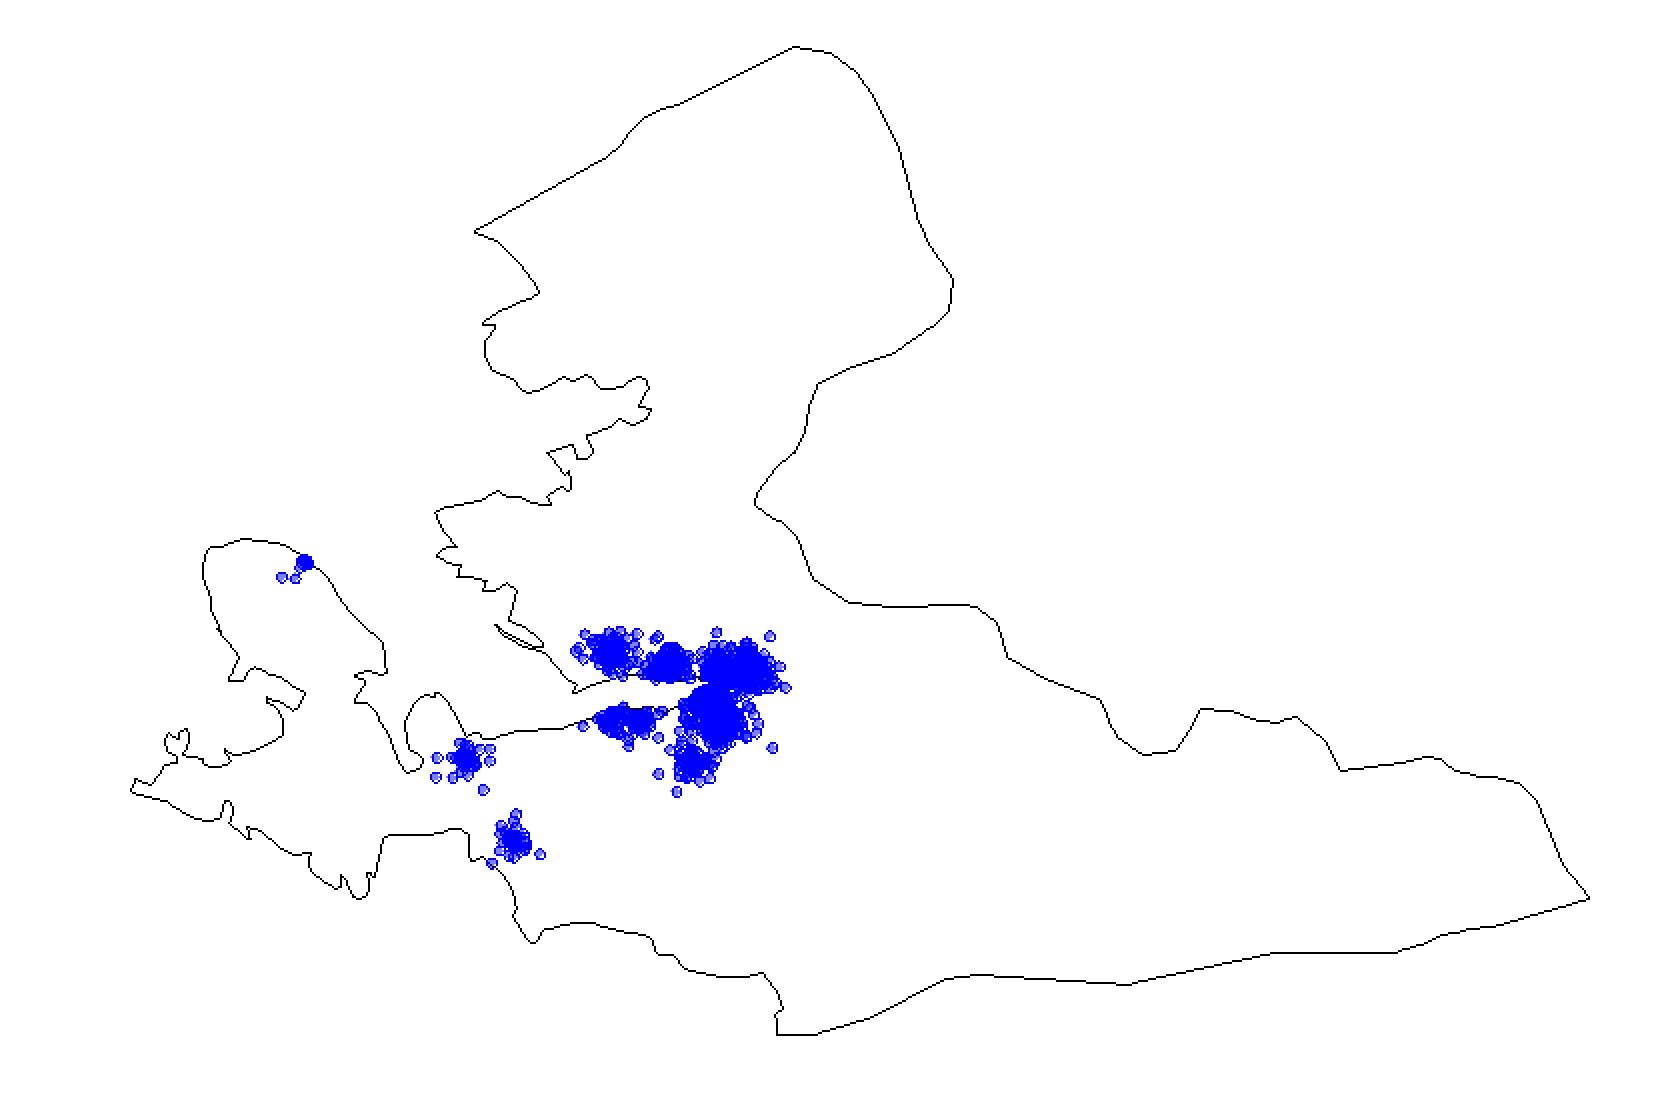
\includegraphics[width=0.8\textwidth]{img/student_map}
\caption{Geographical distribution of student locations in Izmir.}
\label{fig:student_map}
\end{figure}

\subsection{Complete Graph of Transportation Map}
\label{subsec:complete_graph}

A complete graph is the natural mathematical representation of a transportation network where every location is directly connected to every other location. Formally, for our set of student locations $V$, the complete graph $G_{complete} = (V, E_{complete})$ contains an edge $e_{uv} \in E_{complete}$ for every pair of distinct vertices $u, v \in V$, resulting in $|E_{complete}| = {|V| \choose 2} = \frac{|V|(|V|-1)}{2}$ edges. The complete graph connects every pair of distinct student locations, representing maximum potential connectivity as detailed in Section~\ref{se:GraphConstructionMethodsAndSparsity}.

This representation serves as our baseline model, establishing upper bounds on connectivity. However, the dense connectivity often leads to suboptimal routing solutions with higher overall costs due to the ${|V| \choose 2}$ edges making it computationally expensive for large datasets.

\begin{figure}[!htbp]
\centering
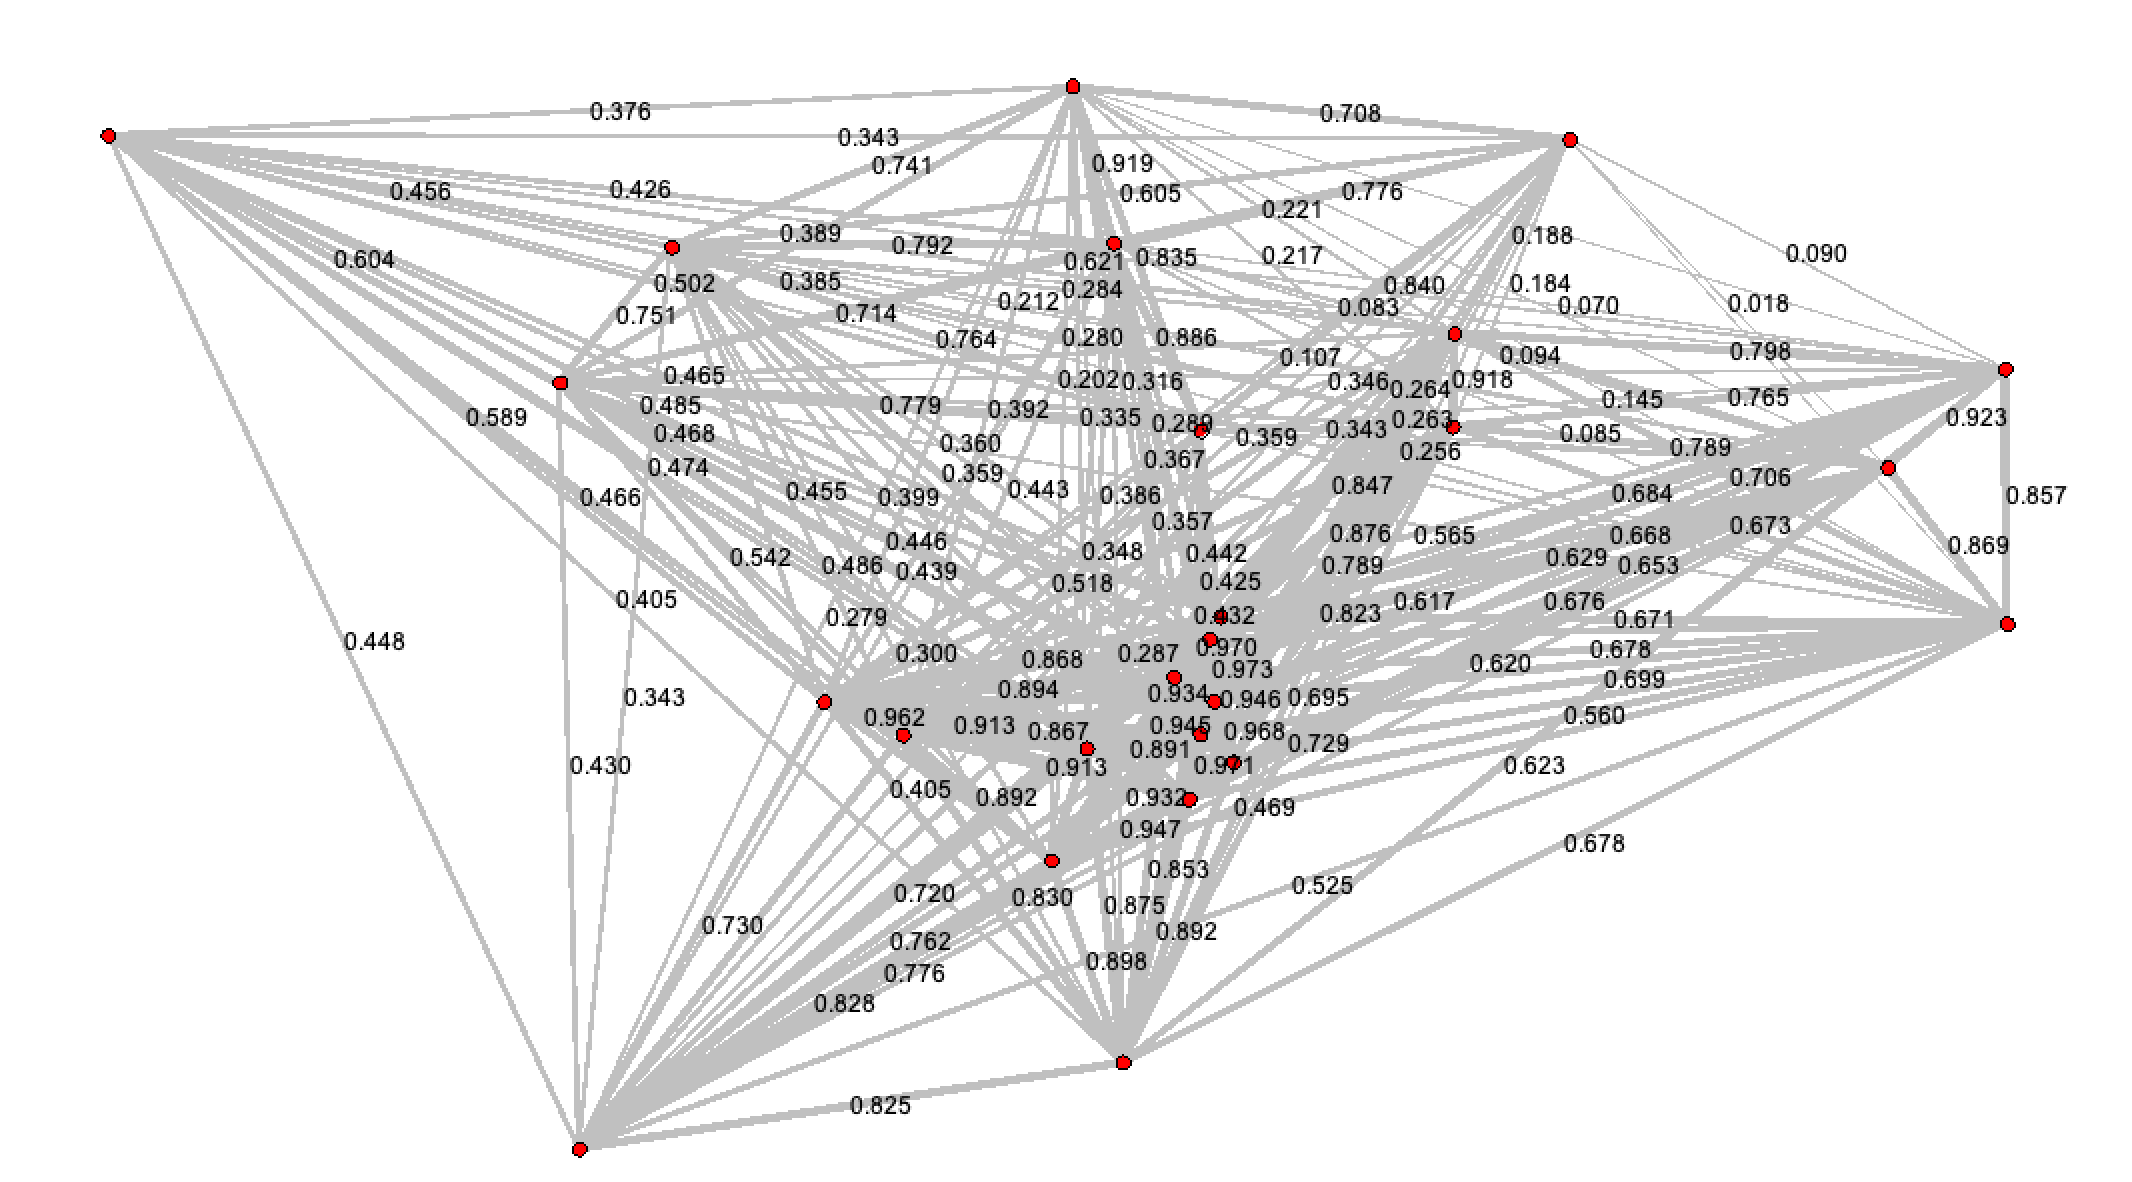
\includegraphics[width=0.6\textwidth]{img/complete}
\caption{Complete graph representation of a sample of student locations. Every point is connected to every other point, representing maximum connectivity but leading to computational challenges for large datasets.}
\label{fig:complete_graph}
\end{figure}



\subsection{Sparse Graph Representation}
\label{subsec:sparse_graph}

Given the computational and practical limitations of the complete graph approach, we explored several sparse graph construction techniques that preserve essential connectivity while significantly reducing the number of edges. These methods emphasize local connections and spatial proximity, resulting in more efficient representations of the transportation network.

\subsubsection{Delaunay Graph Representation}
\label{subsubsec:delaunay}

The Delaunay triangulation constructs a graph $G_{Delaunay}=(V, E_{Delaunay})$ based on the empty circumcircle property as explained in Section~\ref{se:GraphConstructionMethodsAndSparsity}. For any three vertices $p, q, r \in V$, they form a triangle in the Delaunay triangulation if and only if the circumcircle passing through $p, q, r$ contains no other vertex in $V$. This property creates a planar graph that avoids edge crossings and naturally connects proximate points.

\begin{figure}[!htbp]
\centering
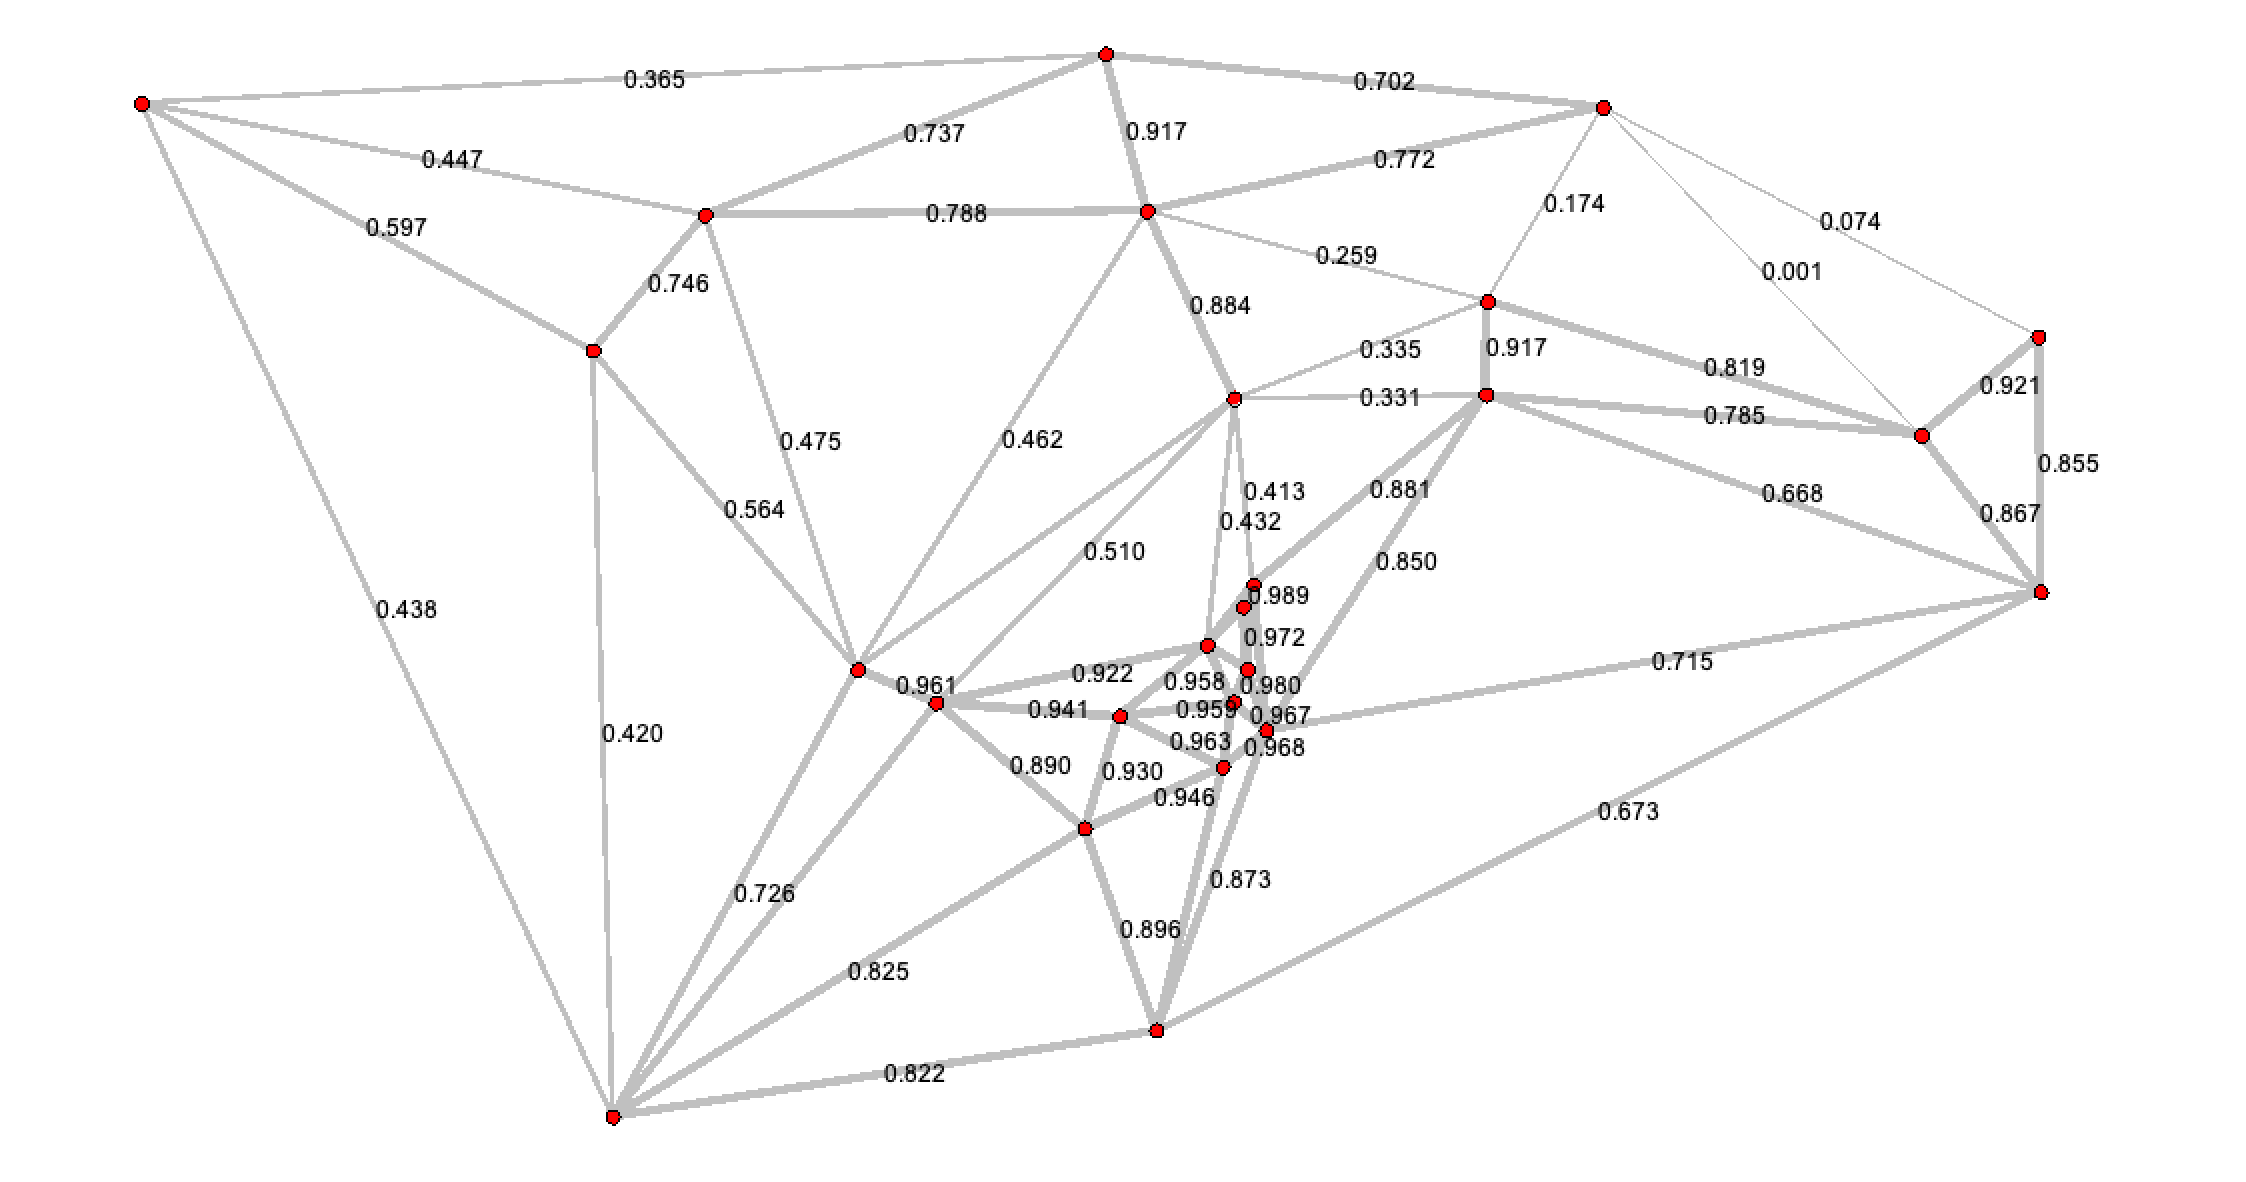
\includegraphics[width=0.6\textwidth]{img/delaunay}
\caption{Delaunay triangulation applied to a sample of student locations. The triangulation connects points such that no point lies inside the circumcircle of any triangle, creating a network that naturally preserves proximity relationships.}
\label{fig:delaunay_graph}
\end{figure}

\subsubsection{Gabriel Graph Representation}
\label{subsubsec:gabriel}

The Gabriel graph is a subgraph of the Delaunay triangulation that connects nodes if the circle with diameter between them contains no other nodes (see Section~\ref{se:GraphConstructionMethodsAndSparsity}). Formally, for our set of student locations $V$, the Gabriel graph $G_{Gabriel}=(V, E_{Gabriel})$ contains an edge $e_{uv} \in E_{Gabriel}$ if and only if:

\begin{equation}
d^2(u, v) < d^2(u, w) + d^2(v, w) \text{ for all } w \in V, w \neq u, w \neq v
\end{equation}

where $d(u, v)$ represents the Euclidean distance between vertices $u$ and $v$.

Our implementation constructs the Gabriel graph by first generating the Delaunay triangulation and then filtering edges based on the empty circle criterion. This approach preserves the most efficient local connections while further reducing the computational complexity compared to the complete graph.

\begin{figure}[!htbp]
\centering
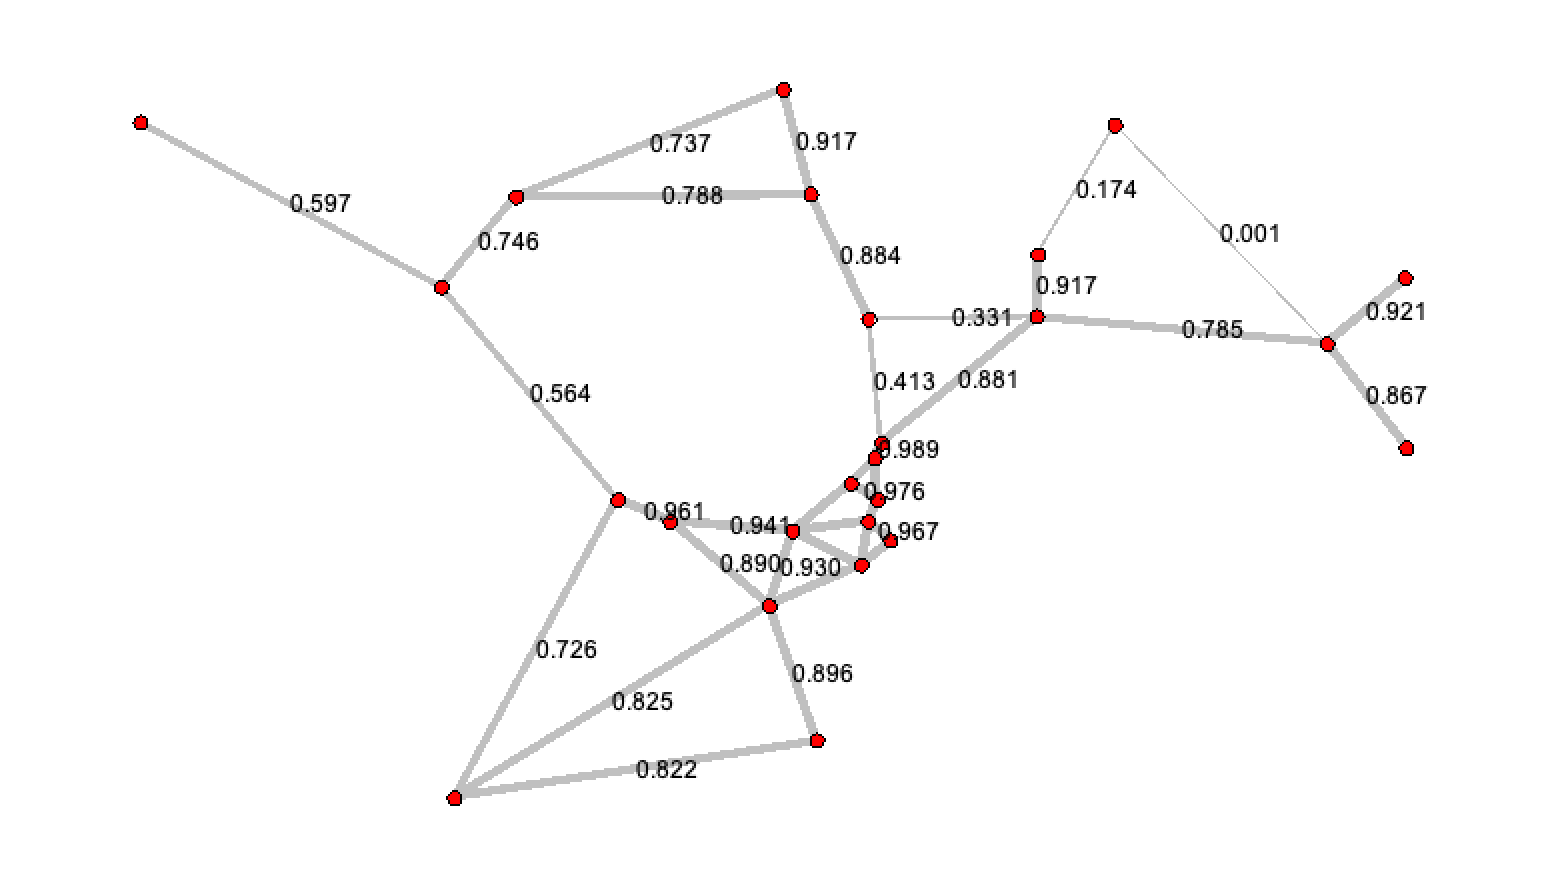
\includegraphics[width=0.6\textwidth]{img/gabriel}
\caption{Gabriel graph derived from student location data. This graph is a subgraph of the Delaunay triangulation, where an edge between two points exists only if the circle with the diameter equal to the distance between them contains no other points.}
\label{fig:gabriel_graph}
\end{figure}

\subsubsection{K-Nearest Neighbour Graph Representation}
\label{subsubsec:knn}

The K-Nearest Neighbors (KNN) graph connects each node to its $k$ closest neighbors, creating a sparse representation that emphasizes local connectivity as detailed in Section~\ref{se:GraphConstructionMethodsAndSparsity}. For our set of student locations $V$, the KNN graph $G_{KNN}=(V, E_{KNN})$ contains edges such that:

\begin{equation}
E_{KNN} = \{(u, v) \mid v \in \text{kNN}(u) \text{ or } u \in \text{kNN}(v)\}
\end{equation}

where $\text{kNN}(u)$ represents the $k$ nearest neighbors of vertex $u$ according to Euclidean distance.

In our implementation, we set $k=30$ based on the average seat size of buses in the IZTECH fleet, ensuring that each node is connected to approximately the number of students that would typically share transportation. The graph is constructed using spatial indexing for efficient neighbor queries, with edge weights based on the Euclidean distance between connected nodes.

\begin{figure}[!htbp]
\centering
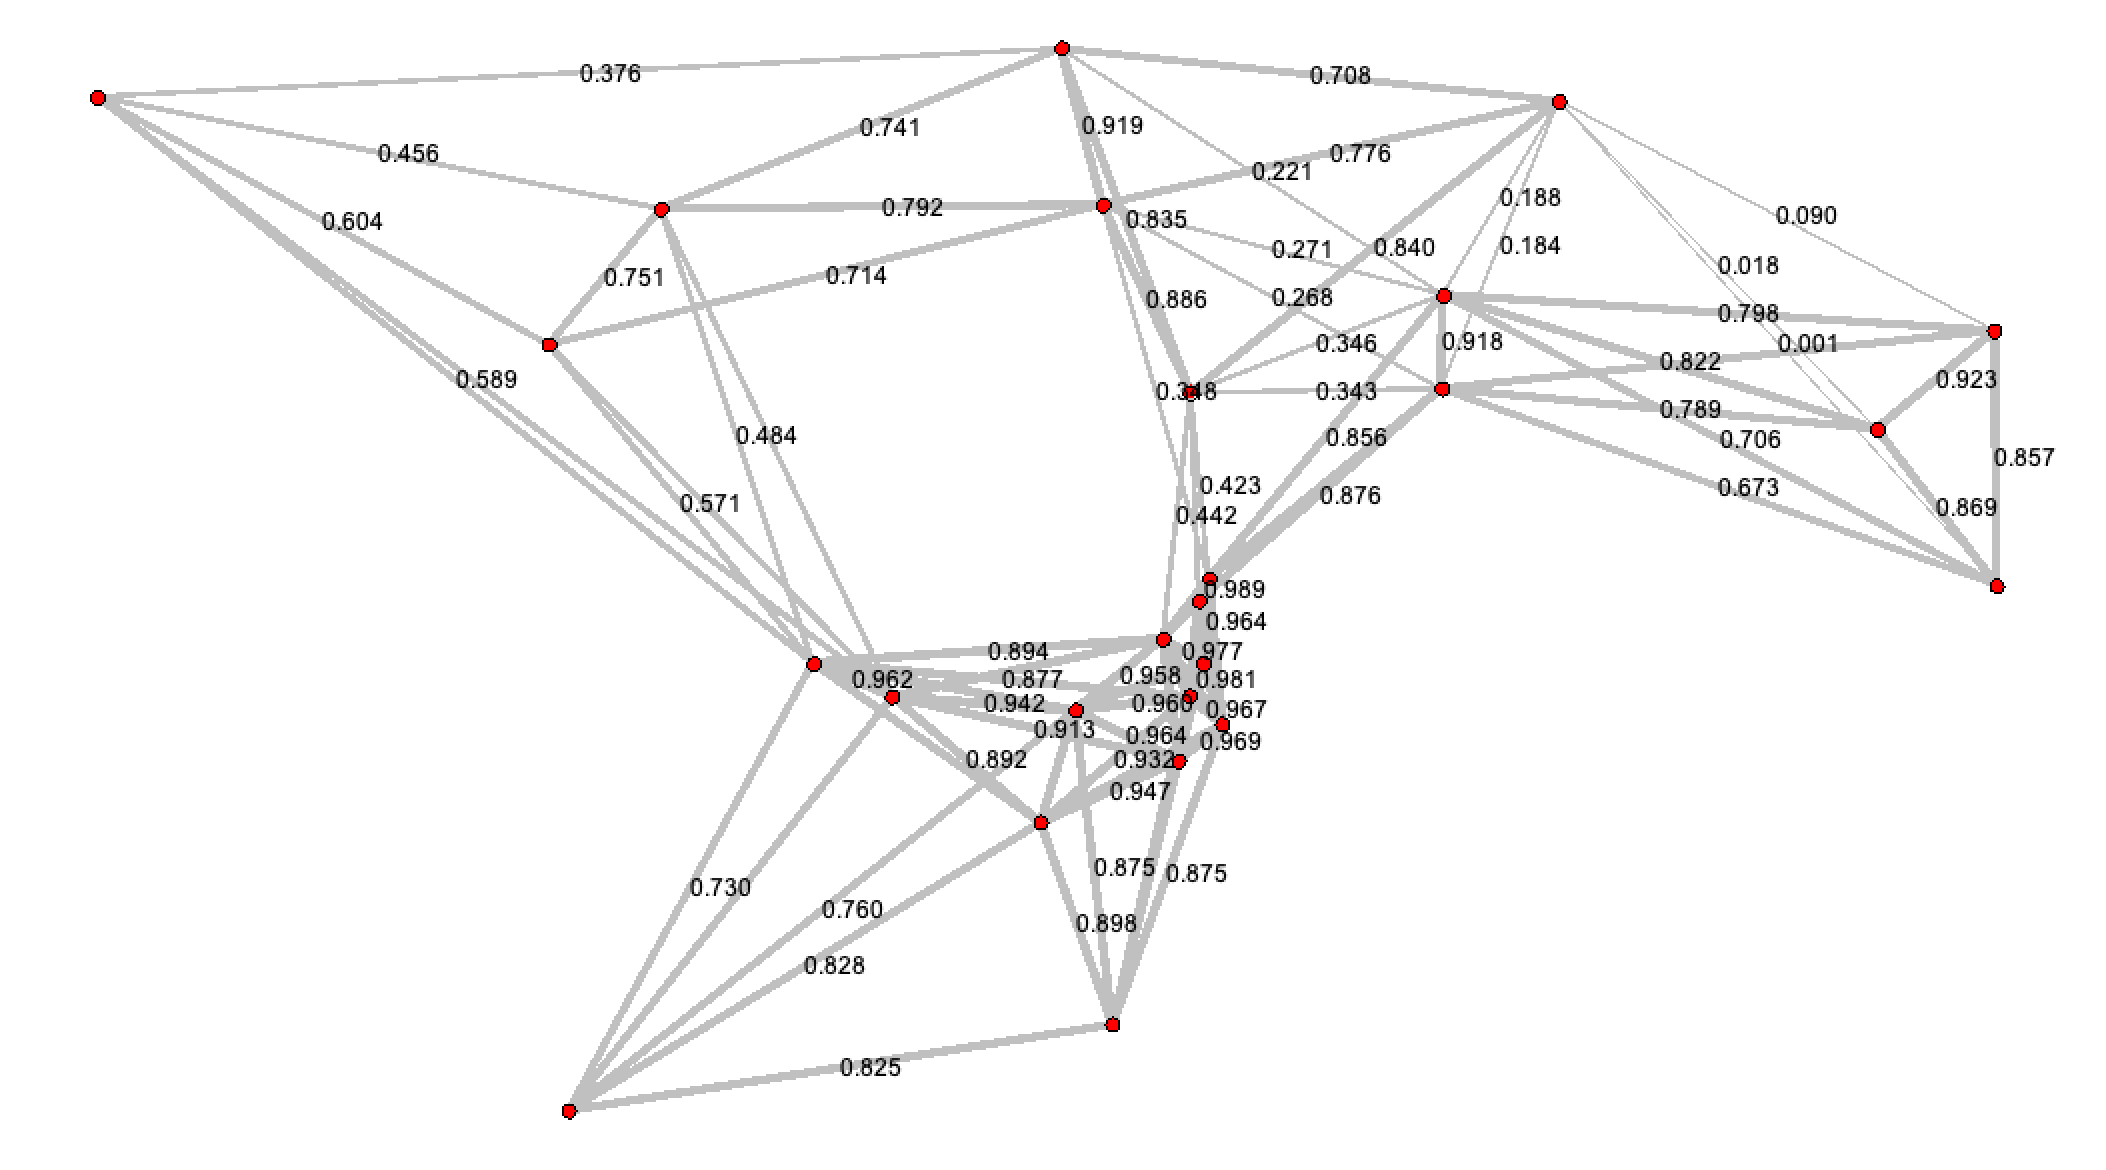
\includegraphics[width=0.6\textwidth]{img/k_nearest}
\caption{K-Nearest Neighbors graph with $k=5$ applied to student location data. Each point is connected to its five closest neighbors, creating a sparse network that preserves local connectivity while significantly reducing the number of edges compared to the complete graph.}
\label{fig:knn_graph}
\end{figure}

\section{Clustering Graph Representation of IZTECH}
\label{sec:clustering_graph}

Once the various graph representations were constructed, we applied clustering algorithms to partition the nodes (students) into clusters, representing potential bus routes. The clustering phase is critical for identifying cohesive groups of students who can be efficiently transported together.

\subsection{Clustering Complete Graph Representation}
\label{subsec:clustering_complete}

Clustering the complete graph representation presents unique challenges due to its dense connectivity. Our implementation applies multiple clustering algorithms to the complete graph, each configured to respect the bus capacity constraints. We enforced a minimum cluster size of 10 students (minimum efficient bus occupancy) and a maximum cluster size of 50 students (maximum bus capacity) to ensure practical viability of the resulting routes.

We primarily utilized the Leiden algorithm (see Section~\ref{subsec:LeidenAlgorithm}), which optimizes modularity to find densely connected communities with its refinement phase ensuring well-connected clusters. The algorithm was configured with adaptive resolution to produce balanced clusters.

\begin{table}[h]
\centering

\label{tab:leiden_complete_example}
\begin{tabular}{|c|c|c|c|c|c|c|c|}
\hline
\textbf{Comm.} & \textbf{Students}  &  \textbf{Distance} & \textbf{Fuel} & \textbf{Fuel Cost} & \textbf{Total} \\
\textbf{ID} & & \textbf{(km)} & \textbf{(L)} & \textbf{(TL)} & \textbf{Cost (TL)} \\
\hline
54 & 18  & 45.70 & 18.74 & 849.35 & 2445.35 \\
\hline
\end{tabular}
\caption{Example of a clustered community using Leiden algorithm on complete graph}
\end{table}

The clusters from the complete graph often required post-processing to merge small communities and split oversized ones, ensuring adherence to the capacity constraints. This post-processing uses geographic proximity to guide the merging and splitting operations, prioritizing the combination of communities that are spatially close while ensuring each resulting community remains within the capacity limits.

\subsubsection{Minibus Solution for Imbalanced Clusters}
\label{subsubsec:minibus_solution}

When analyzing the complete graph representation, we observed that the resulting clusters were often imbalanced, with many clusters having fewer than 25 students. This created an inefficiency in the transportation system, as standard buses with a capacity of 50 students would be underutilized. To address this issue, we implemented a vehicle type allocation strategy that assigns minibuses (with a maximum capacity of 25 students) to smaller clusters containing 10-25 students, while standard buses were allocated to larger clusters with 26-50 students. This differentiated approach resulted in significant cost savings due to the lower fuel consumption of minibuses compared to standard buses. However, it's important to note that IZTECH currently does not have minibuses in its fleet, only standard buses. This limitation motivates our exploration of alternative graph construction methods that might produce more balanced clusters suitable for the existing bus fleet.

\subsection{Clustering Sparse Graph Representation}
\label{subsec:clustering_sparse}

The sparse graph representations required different clustering approaches due to their reduced connectivity. Our implementation adaptively configures the clustering algorithms based on the graph type.

For Delaunay and Gabriel graphs, we utilized the Spectral clustering algorithm (see Section~\ref{subsec:SpectralClustering}), which uses the eigenvalues and eigenvectors of the graph Laplacian to perform dimensionality reduction before clustering.

For the K-Nearest Neighbors graph, we found that the MVAGC (Multi-view Anchor Graph-based Clustering) algorithm performed especially well. As described in Section~\ref{subsec:MVAGC}, this algorithm constructs multiple views of the graph and integrates them through an anchor graph representation. Our configuration included approximately 500 anchor points, higher-order filtering for smooth community boundaries, and importance sampling to improve anchor diversity.

All clustering approaches were evaluated based on their ability to produce balanced clusters that minimize transportation costs while adhering to the vehicle capacity constraints.

% Placeholder for Clustering Example Visualization
\begin{figure}[!htbp]
\centering
\subfigure[Spectral Clustering]{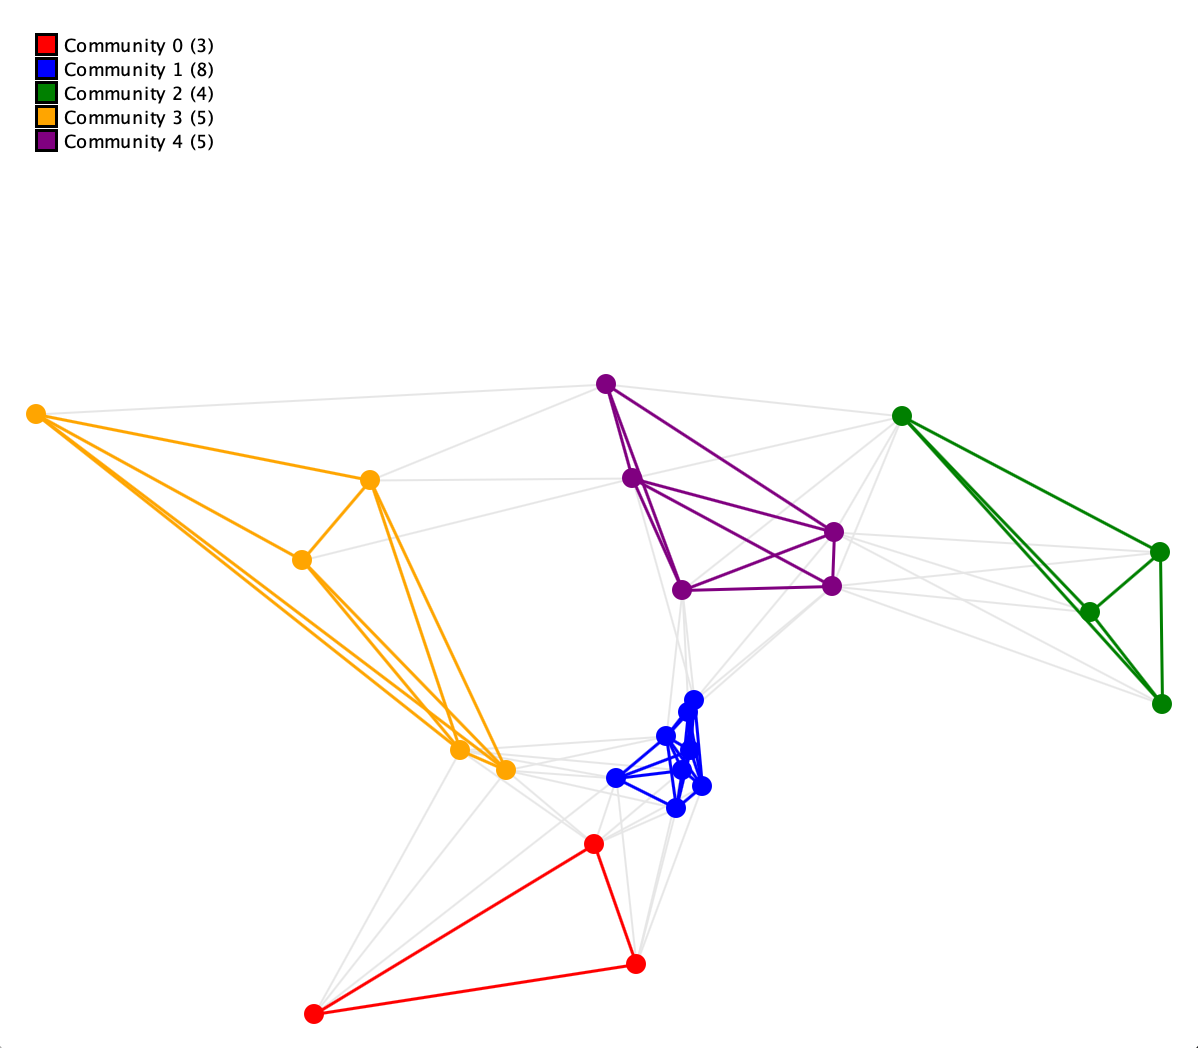
\includegraphics[width=0.32\textwidth]{img/spectral}}
\subfigure[Leiden Algorithm]{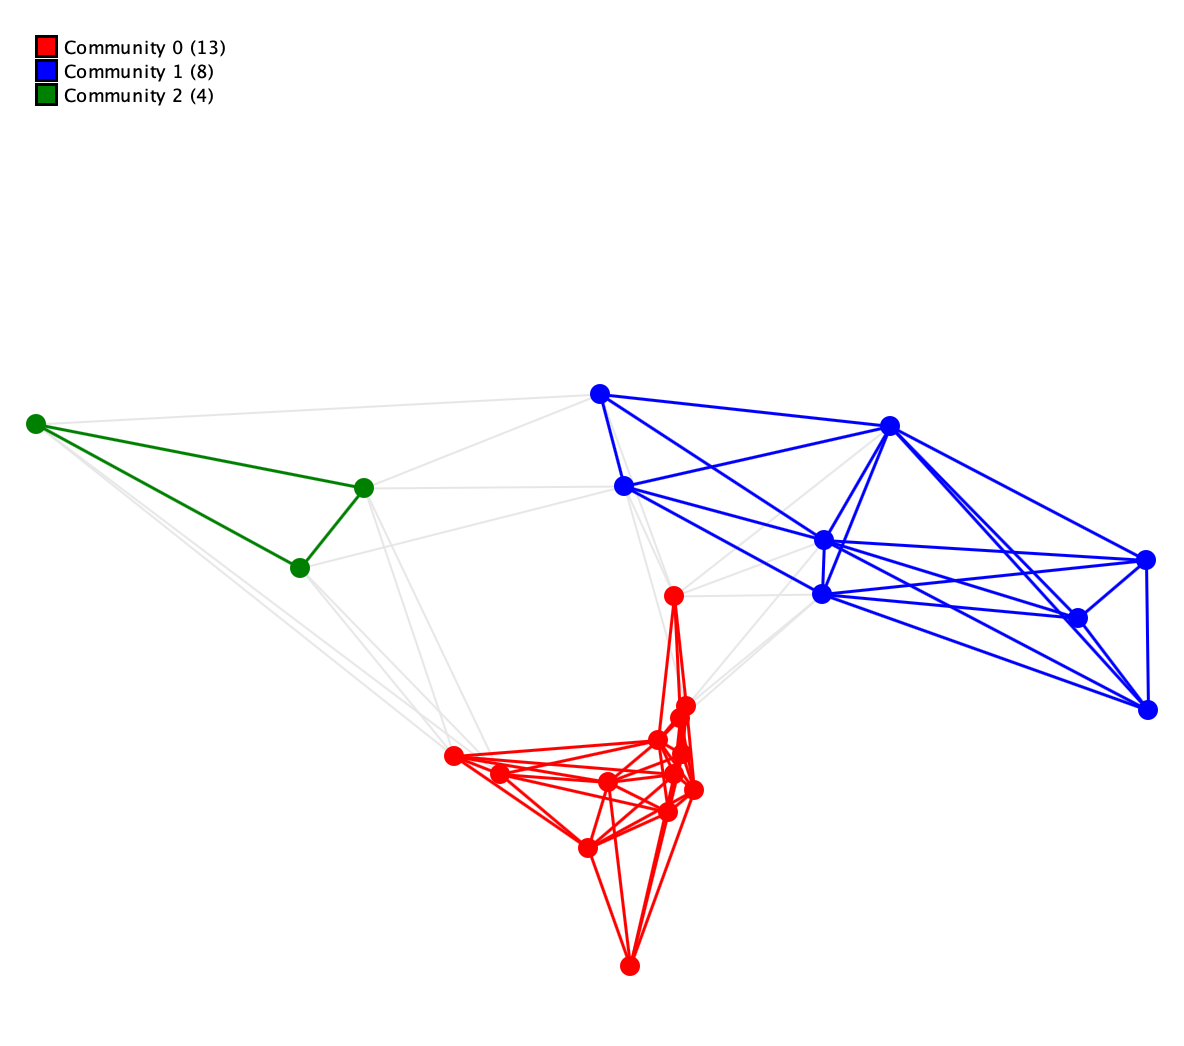
\includegraphics[width=0.32\textwidth]{img/leiden}}
\subfigure[MVAGC]{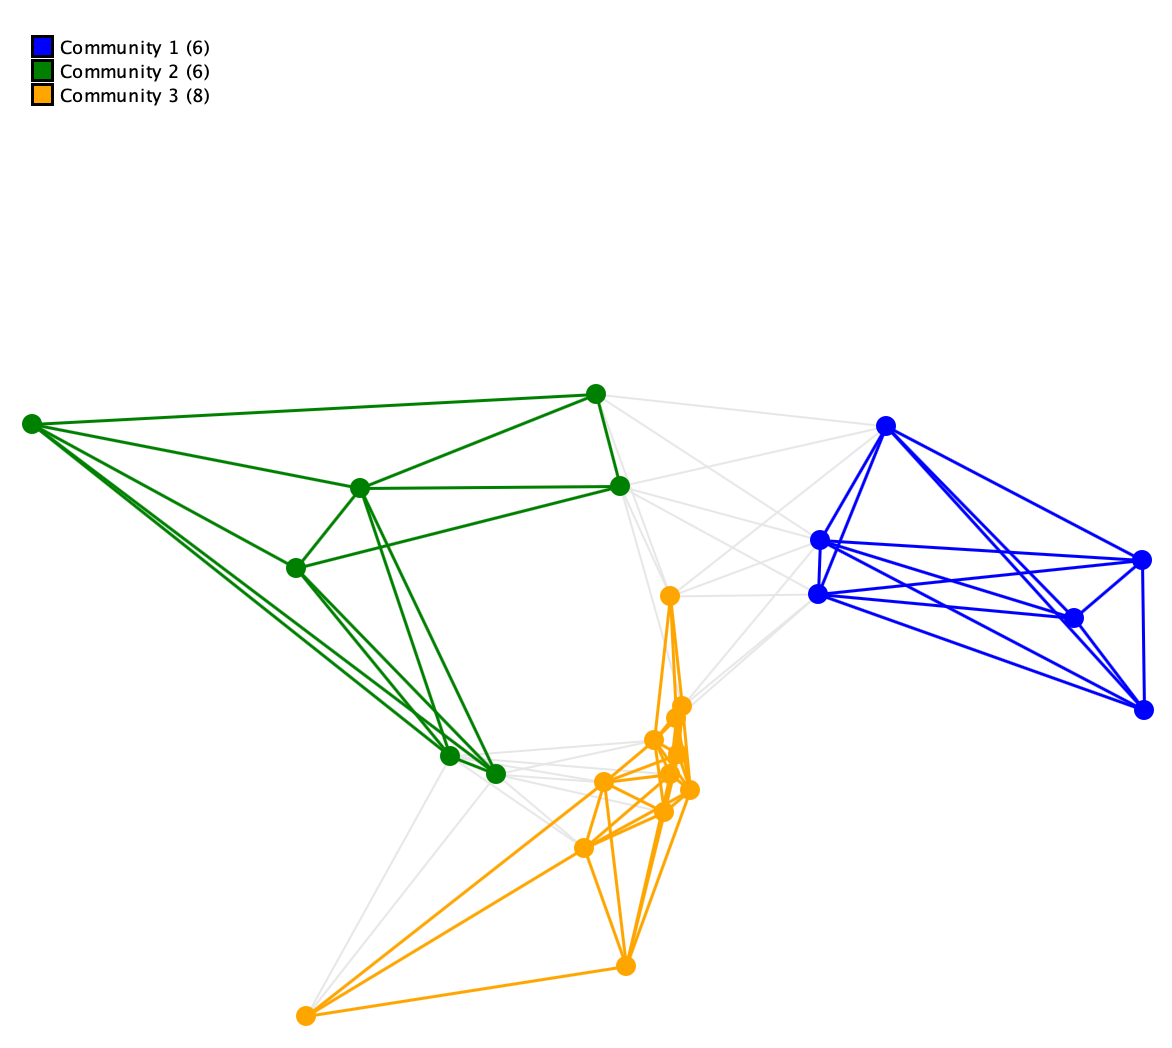
\includegraphics[width=0.32\textwidth]{img/mvagc}}
\caption{Results of applying different clustering algorithms to the graph representations. Each color represents a distinct cluster of student locations, corresponding to potential bus routes prior to capacity constraint adjustments.}
\label{fig:clustering_example}
\end{figure}

\section{Robustness for Clustering Graph Representation of IZTECH}
\label{sec:robustness}

% Commenting out the example algorithm from the template
% \begin{algorithm}
% \begin{algorithmic}[1]
% \STATE generate random number $n \in [l, u]$
% \WHILE{$n \neq 42$}
% \IF{today is Tuesday}
% \STATE print(42)
% \ENDIF
% \ENDWHILE
% \RETURN best solution found so far
% \end{algorithmic}
% \caption{Basic Algorithm($l, u$)}
% \label{alg:example_alg}
% \end{algorithm}



